\documentclass[12pt, oneside]{book}

% Encoding and Font Packages
\usepackage[T1]{fontenc} % Enables more efficient encoding for characters
\usepackage[utf8]{inputenc} % Allows for direct input of Unicode characters
\usepackage{microtype} % Improves typography by fine-tuning text spacing

% Font Setup for Official Text
\usepackage{charter} % Primary font for readability
\usepackage{bm} 
\usepackage{mathpazo} 

% Monospaced Font for Code Listings
\usepackage[scaled=.95]{inconsolata}

% Color and Graphics
\usepackage{array}
\usepackage{xcolor} % For custom color definitions
\usepackage{graphicx} % To insert images, diagrams, etc.
\usepackage{caption} % Customization of figure captions
\usepackage{subcaption} % For sub-figures (helpful for detailed diagrams)
\usepackage{tikz} % For high-quality, custom diagrams and illustrations
\usetikzlibrary{positioning, shapes.geometric, arrows, calc} % Libraries for complex diagram creation

% Margins and Page Layout
\usepackage[a4paper, margin=1in]{geometry} % Adjust page margins
\usepackage{setspace} % For line spacing
\setstretch{1.3} % Sets a nice line spacing for the text (readable and clear)

% Headers and Footers
\usepackage{fancyhdr} % For fancy headers and footers
\pagestyle{fancy}
\fancyhf{}
\fancyhead[L]{\nouppercase{\leftmark}} % Left-aligned chapter heading
\fancyhead[R]{\thepage} % Right-aligned page number
\fancypagestyle{plain}{
	\fancyhf{}
	\fancyfoot[C]{\thepage} % Centered page number for "plain" pages
}

% Hyperlink and Navigation
\usepackage{hyperref} % For hyperlinks and navigation within the document
\hypersetup{
	colorlinks=true, % Enables colored links
	linkcolor=black, % Links are in black (good for printing)
	citecolor=blue, % Citation links are blue
	urlcolor=cyan, % URLs are cyan
	pdfauthor={Mahdi}, % Author metadata for PDF
	pdftitle={Arliz}, % Title metadata for PDF
	pdfsubject={Programming, Arrays, and Data Structures}, % Subject for PDF
	pdfkeywords={Arrays, Data Structures, Programming, History of Computing}, % Keywords for PDF
}

% Bibliography
\usepackage[backend=biber,style=apa]{biblatex} % APA-style citations
\addbibresource{references.bib} % Add the bibliography file

% Listings for Code
\usepackage{listings} % For code listings and syntax highlighting
\lstset{
	basicstyle=\ttfamily\small, % Monospaced font for code
	frame=single, % Draws a box around the code block
	breaklines=true, % Automatically breaks lines in code
	numbers=left, % Line numbers on the left
	numberstyle=\tiny\color{gray}, % Style of line numbers
	keywordstyle=\color{myblue}\bfseries, % Keywords in blue and bold
	commentstyle=\color{olive}, % Comments in green
	stringstyle=\color{orange}, % Strings in orange
	backgroundcolor=\color{lightgray!20}, % Light background for code blocks
	captionpos=b, % Position the caption at the bottom
	escapeinside={(*@}{@*)}, % Allows for inline LaTeX inside code blocks
	morekeywords={array, structure, algorithm, complexity}, % Add relevant keywords for highlighting
}

% Table of Contents and Index
\usepackage{tocbibind} % Adds bibliography and index to the table of contents
\usepackage{imakeidx} % For index generation
\makeindex % Generates the index

% Title Customization
\usepackage{titlesec} % For customizing chapter and section styles
\titleformat{\chapter}[display]
{\normalfont\huge\bfseries}{\chaptername\ \thechapter}{20pt}{\Huge}
\titleformat{\section}{\Large\bfseries}{\thesection}{1em}{}
\titleformat{\subsection}{\large\bfseries}{\thesubsection}{1em}{}

% Algorithms and Pseudocode
\usepackage{algorithm} % For displaying algorithms
\usepackage{algpseudocode} % For pseudocode formatting

% Multicolumn for Glossary or Index
\usepackage{multicol} % For multicolumn layouts (useful for glossary)

% Custom Colors
\definecolor{myblue}{RGB}{0, 102, 204} % Define a custom blue color for code and links
\definecolor{lightgray}{RGB}{240, 240, 240} % Light gray for code backgrounds

% Title and author
\title{{\Huge Arliz}} % Book title (Large font)
\author{{\LARGE Mahdi}} % Author name (Large font)
\date{{\large \today}} % Date of the document

\begin{document}
	\frontmatter
	\mainmatter
	\maketitle
	\tableofcontents
	\renewcommand{\arraystretch}{1.5} % Adjust row height for better readability
	
	\section{Preface}
	\addcontentsline{toc}{chapter}{Preface}
	
	Every book has its own story, and this book is no exception. If I were to summarize the process of creating this book in one word, that word would be “improvised.” Yet the truth is that Arliz is the result of pure, persistent curiosity that has grown in my mind for years. What you are reading now could be called a technical book, a collection of personal notes, or even a journal of unanswered questions and curiosities. But I—officially—call it a \emph{book}, because it is written not only for others but for myself, as a record of my learning journey and an effort to understand more precisely the concepts that once seemed obscure and, at times, frustrating.\\
	The story of Arliz began with a simple feeling: \textbf{curiosity}.  
	Curiosity about what an array truly is. Perhaps for many this question seems trivial, but for me this word—encountered again and again in algorithm and data structure discussions—always raised a persistent question.\\
	Every time I saw terms like \texttt{array}, \texttt{stack}, \texttt{queue}, \texttt{linked list}, \texttt{hash table}, or \texttt{heap}, I not only felt confused but sensed that something fundamental was missing. It was as if a key piece of the puzzle had been left out. The first brief, straightforward explanations I found in various sources never sufficed; they assumed you already knew exactly what an array is and why you should use it. But I was looking for the \emph{roots}. I wanted to understand from zero what an array means, how it was born, and what hidden capacities it holds.\\
	That realization led me to decide:  
	\emph{If I truly want to understand, I must start from zero.}\\	
	There is no deeper story behind the name “Arliz.” There is no hidden philosophy or special inspiration—just a random choice. I simply declared:  
	\emph{This book is called Arliz.}  
	You may pronounce it “Ar-liz,” “Array-ees,” or any way you like. I personally say “ar-liz.” That is all—simple and arbitrary.\\	
	But Arliz is not merely a technical book on data structures. In fact, \textbf{Arliz grows alongside me}. \\
	Whenever I learn something I deem worth writing, I add it to this book. Whenever I feel a section could be explained better or more precisely, I revise it. Whenever a new idea strikes me—an algorithm, an exercise, or even a simple diagram to clarify a structure—I incorporate it into Arliz.\\
	This means Arliz is a living project. As long as I keep learning, Arliz will remain alive.\\	
	In writing this book, I have always tried to follow three principles:
	
	\begin{itemize}
		\item \textbf{Simplicity of Expression:} I strive to present concepts in the simplest form possible, so they are accessible to beginners and not superficial or tedious for experienced readers.
		\item \textbf{Concept Visualization:} I use diagrams, figures, and visual examples to explain ideas that are hard to imagine, because I believe visual understanding has great staying power.
		\item \textbf{Clear Code and Pseudocode:} Nearly every topic is accompanied by code that can be easily translated into major languages like C\texttt{++}, Java, or C\#, aiming for both clarity and practicality.
	\end{itemize}
	
	An important note: many of the algorithms in Arliz are implemented by myself. I did not copy them from elsewhere, nor are they necessarily the most optimized versions. My goal has been to understand and build them from scratch rather than memorize ready-made solutions. Therefore, some may run slower than standard implementations—or sometimes even faster. For me, the process of understanding and constructing has been more important than simply reaching the fastest result.\\	
	Finally, let me tell you a bit about myself:  
	I am \textbf{Mehdi}. If you prefer, you can call me by my alias: \emph{Genix}. I am a student of Computer Engineering (at least at the time of writing this). I grew up with computers—from simple games to typing commands in the terminal—and I have always wondered what lies behind this screen of black and green text. There is not much you need to know about me, just that I am someone who works with computers, sometimes gives them commands, and sometimes learns from them.\\	
	I hope this book will be useful for understanding concepts, beginning your learning journey, or diving deeper into data structures. \\	
	Arliz is freely available. You can access the PDF, LaTeX source, and related code at:  
	\begin{center}
		\url{https://github.com/m-mdy-m/Arliz}
	\end{center}
	In each chapter, I have included exercises and projects to aid your understanding. Please do not move on until you have completed these exercises, because true learning happens only by solving problems.\\	
	I hope this book serves you well—whether for starting out, reviewing, or simply satisfying your curiosity. And if you learn something, find an error, or have a suggestion, please let me know. As I said:
	\emph{This book grows with me.}
	
	% Acknowledgments
	\chapter*{Acknowledgments}
	\addcontentsline{toc}{chapter}{Acknowledgments}
	I would like to express my gratitude to everyone who supported me during the creation of this book. Special thanks to the open-source community for their invaluable resources and to all those who reviewed early drafts and provided feedback.
		
	% Main Content
	\mainmatter
	\chapter{Introduction to Arrays}
	
	\section{Overview}
	Arrays are one of the most fundamental data structures in computer science, playing a pivotal role in the organization and manipulation of data. Simply put, an array is a collection of elements, all of the same data type, arranged in a specific order and stored in contiguous memory locations. This simplicity is what makes arrays incredibly versatile—they are not just used in programming but are a concept deeply rooted in mathematics and everyday life.\\
	To illustrate, imagine a multi-story building. Each floor, stacked one on top of the other, represents a single element in an array, while the entire building symbolizes the array itself. Or think of the rows and columns in a calendar—they mimic a two-dimensional array where the rows represent weeks and the columns represent days.\\
	In computer science, arrays act as the backbone for more advanced data structures and algorithms. They are a starting point for understanding complex concepts like matrices, heaps, or even artificial intelligence models. Whether you’re sorting data, managing game levels, or storing large datasets, arrays provide a way to organize and access information efficiently.\\
	Arrays also have a significant impact outside programming. In mathematics, arrays manifest as lists, sets, or matrices, helping solve equations and model systems. In engineering, arrays are used to simulate real-world phenomena, such as simulating airflow over a car body or rendering graphics in a video game. These real-world analogies highlight the universality of arrays, bridging the gap between abstract computation and tangible applications.\\
	Why are arrays so important? It’s because they allow for direct access to elements using an index. This makes operations like reading, writing, or modifying data fast and predictable—qualities essential for performance-critical applications. From a programmer’s perspective, arrays simplify data handling, reduce memory overhead, and enable powerful algorithms like binary search or quicksort.\\
	This chapter introduces you to the world of arrays, their origins, and their significance in both historical and modern contexts. By exploring their structure, purpose, and usage, you will uncover how arrays lay the foundation for efficient data storage, processing, and computation. Whether you're a beginner programmer curious about data organization or an experienced developer refining your knowledge, mastering arrays is a cornerstone of software development.\\
	In the chapters that follow, we’ll delve into the history of arrays, trace their evolution in programming languages, and examine their profound influence on computer architecture. By starting with this foundational concept, you’re setting the stage for a deeper understanding of how computers work and how data flows through software systems. Let’s explore the power and elegance of arrays together!
	\section{Why Use Arrays?}
	As discussed in the previous section, one of the primary reasons for using arrays is their ability to provide fast access to individual elements. Imagine a 100-story building where each floor represents an element in an array. If you want to go straight to the 99th or 100th floor, you can do so instantly, just like Superman soaring directly to the top. This efficiency is a hallmark of arrays—they allow you to access any element directly by its index without needing to traverse the entire structure.\\
	However, fast access is just one of the many reasons why arrays are indispensable. Arrays are not only the simplest but also the oldest data structure in computer science. Their simplicity is a significant advantage, making them easy to implement and universally supported in virtually all programming languages and systems. Whether you're working with low-level assembly code or a high-level language like Python, arrays are a fundamental feature.\\
	Another compelling reason to use arrays is their speed. Arrays provide constant-time (O(1)) access to elements, making them extremely fast for read and write operations when the index is known. This efficiency has contributed to their popularity and widespread use in various computational tasks.\\
	Arrays are also incredibly flexible. They can be used to represent and manipulate almost any type of data. For instance:\\
	\begin{itemize}
		\item The text you are reading right now is stored and displayed as an array of characters. Each letter, space, or symbol is an element in that array.
		\item Your phone or computer screen is essentially a 2D array (or matrix) of pixels. Each pixel has an (x, y) coordinate and a corresponding color value. Arrays allow computers to organize and manipulate these elements, enabling the display of text, images, and graphical interfaces.
	\end{itemize}
	In essence, arrays serve as the backbone for countless operations in computing, from handling raw data to building sophisticated algorithms and systems. Their combination of simplicity, speed, and versatility makes them one of the most practical and essential tools in computer science. Whether you're a novice or an experienced developer, mastering arrays is a crucial step in understanding how computers store and process information. 
	\section{History}
	The history and concept of arrays as a data structure are deeply embedded in the evolution of computing, tracing back to the era of the first digital computers. If the entire history of arrays were to be summarized in one sentence, it might be this: 
	\begin{quote}
		\textit{"Arrays have not only shaped the way we organize and process data but have also significantly influenced—and continue to influence—the design and development of programming languages and computer architecture."}
	\end{quote}
	Arrays, one of the simplest yet most foundational data structures in computer science, have a rich history that intertwines with advancements in mathematics, computing, and programming languages. Born from the necessity to organize and process data efficiently, they have evolved in parallel with breakthroughs in computer architecture and software development. \\
	The journey of arrays is a testament to innovation and problem-solving, reflecting their central role in shaping how we approach data storage and manipulation. From the earliest mathematical concepts to their critical role in algorithms and modern programming languages, arrays have been at the heart of data organization. Their origins, development, and widespread adoption provide a compelling glimpse into the broader progression of computing and its relentless push toward efficiency and scalability.
	\subsection{Origins and Necessity of Arrays}
	The concept of arrays originated from the need to manage and manipulate large volumes of data efficiently. The word "array" itself, meaning an orderly arrangement, is apt, as arrays in computing serve to organize data elements of the same type in a structured, sequential manner. The earliest inspiration for arrays comes from mathematics, where arrays functioned as vectors or matrices to perform complex mathematical operations. Mathematicians had long relied on arrays in tabular form to represent and compute large datasets. However, it wasn’t until the advent of mechanical and electromechanical computing devices in the late 19th and early 20th centuries that arrays began to take on a computational form. \\ As early computing systems emerged, especially those performing repetitive or large-scale calculations, there was a clear requirement for a structure that could handle collections of similar data elements. Arrays provided a solution by offering a systematic way to store data in contiguous memory locations, enabling quick access and manipulation.\\The first practical implementations of arrays can be traced back to the late 19th and early 20th centuries with the advent of mechanical and electromechanical computing devices. One of the earliest forms of arrays was seen in \href{https://en.wikipedia.org/wiki/Punched_card}{the punch card} systems, where data was organized in a tabular format. Each row in these tables could be considered an early version of an array, with each column representing different data fields. Hollerith's punch card system, for example, allowed data to be stored in a tabular form, where rows and columns resembled the layout of a modern array. While rudimentary, this approach provided a glimpse of the systematic storage and access principles that would define arrays in computing. However, the modern conceptualization of arrays truly began to take shape with the advent of digital computers in the 1940s.
	\subsection{Early Digital Computers}
	During the 1940s, the first digital computers, such as the \href{https://en.wikipedia.org/wiki/ENIAC}{ENIAC} (Electronic Numerical Integrator and Computer) and the Harvard Mark I, were developed primarily for scientific and engineering applications. These early machines were designed to perform complex calculations, and arrays played a crucial role in organizing and manipulating data. However, the programming methods and languages used during this era were quite rudimentary compared to modern standards.\\Programming these early computers was mostly done in machine language or through plugboards (in the case of the ENIAC), where instructions were hardwired into the machine. These methods required programmers to manage arrays manually, including calculating each element's memory address and writing out explicit instructions for operations such as iteration, sorting, and searching. The task was labor-intensive, and coding errors could easily occur due to the complexity of managing data at such a low level.\\However, by the late 1940s and early 1950s, assembly language started to emerge, providing a slightly higher level of abstraction for programming. Assembly language allowed symbolic representation of machine code instructions, making it somewhat easier to work with arrays and other data structures. Even then, programmers still had to manage many of the details manually, such as addressing and looping through array elements. For example, to access the 10th element of an array, programmers needed to know the memory address of the first element and calculate the offset.  \\One notable development during this period was the creation of the EDSAC (Electronic Delay Storage Automatic Calculator) in 1949, which was one of the first computers to use a stored-program architecture. The EDSAC ran the first stored program on May 6, 1949, and this architecture allowed both data and instructions to be stored in the same memory. While programming was still done in assembly language, the stored-program concept laid the groundwork for more advanced programming techniques and languages that would emerge in the following decade.\\The limited memory and processing power of these early computers made arrays essential for optimizing performance. Arrays allowed programmers to store data sequentially, reducing the overhead associated with data access and manipulation, and made efficient use of the available memory. Despite the primitive programming tools, arrays were indispensable for tasks like solving systems of linear equations, performing numerical simulations, and managing large datasets in statistical computations, all of which were common in the scientific and engineering calculations for which these early machines were used.
	\subsection{The Influence of John von Neumann}
	A figure in the history of arrays is the renowned mathematician and computer scientist, \href{https://en.wikipedia.org/wiki/John_von_Neumann#Computer_science}{John von Neumann}. In 1945, von Neumann made significant contributions to the development of the first stored-program computers, where both instructions and data were stored in the same memory. This innovation allowed for more flexible and powerful computational systems.\\One of von Neumann's notable achievements was the creation of the first array-sorting algorithm, known as \textbf{mergesort}. This algorithm efficiently organizes data in an array by dividing the array into smaller sub-arrays, sorting them, and then merging them back together. The merge sort algorithm laid the groundwork for many subsequent sorting techniques and is still widely used today due to its optimal performance in various scenarios.\\Von Neumann’s work on merge sort and his overall contributions to computer architecture and programming set the stage for the development of high-level programming languages. These languages abstracted the complexity of managing arrays, allowing programmers to focus more on algorithmic development rather than low-level memory management.
	As programming languages evolved from assembly to higher-level languages in the 1950s and 1960s, the concept of arrays became more formalized and easier to use. Languages like Fortran (1957) and COBOL (1959) introduced built-in support for arrays, enabling programmers to declare and manipulate arrays directly without concerning themselves with the underlying memory management.\\This evolution continued with languages such as C, which provided more advanced features for working with arrays, including multi-dimensional arrays and pointers, giving programmers powerful tools for managing data efficiently. Modern programming languages like Python, Java, and C++ further abstract the concept of arrays, offering dynamic array structures like lists and vectors, which automatically handle resizing and memory allocation.
	\subsection{Impact on Computer Architecture}
	The introduction and widespread use of arrays have significantly influenced computer architecture. Arrays demand efficient memory access patterns, leading to advancements in memory hierarchies, cache design, and data locality optimizations. Concepts like \textbf{row-major} and \textbf{column-major} ordering were developed to improve the performance of array operations, particularly for multi-dimensional arrays used in scientific and engineering applications.\\
	The rise of vector processors in the 1970s and 1980s, and later, parallel computing architectures, was driven by the need to process arrays more efficiently. These systems enabled simultaneous operations on multiple array elements, dramatically accelerating tasks like matrix multiplication, image processing, and simulations.\\
	\subsection{A Lasting Legacy}
	From their origins in mathematical concepts to their integral role in modern computing, arrays have remained a cornerstone of data organization and processing. They continue to evolve alongside advancements in technology, adapting to new challenges like handling massive datasets in machine learning and optimizing performance for high-performance computing.\\
	Arrays have not just shaped programming and algorithms; they have also influenced how we design and understand computational systems. As we move into fields like quantum computing and bioinformatics, the foundational principles of arrays remain as relevant and transformative as ever.
	\section{Structure and Characteristics of Arrays}
	Now that we know what arrays are and how they came to be, let’s delve deeper into their structure and explore why they are indispensable in programming. While each aspect of arrays has its own chapter for detailed discussion, we’ll summarize key points here as an introduction. Keep these ideas in mind—they'll serve as a foundation for understanding arrays as we progress through this text.\\
	Arrays are more than just collections of elements. They are carefully structured data constructs, designed to optimize both performance and resource utilization. By employing a sequential memory layout, arrays enable rapid and predictable data access. This layout not only allows for efficient retrieval of elements but also ensures that operations on arrays remain consistent and manageable in terms of memory consumption.\\
	Key attributes of arrays include their inherent simplicity, systematic memory arrangement, and direct access capabilities. These features make them one of the most versatile and widely used data structures across programming paradigms. Additionally, arrays provide the foundational building blocks for more complex data structures, such as matrices, tensors, and various types of lists.\\
	In the chapters ahead, we will examine these characteristics in detail, along with practical examples and advanced applications. For now, consider arrays as a powerful tool in computational problem-solving, their utility stemming from a combination of elegance, efficiency, and reliability.
	\subsection{Contiguous Memory Layout}
	To fully appreciate the power and efficiency of arrays, it’s essential to understand how they are stored in memory. Arrays rely on a **contiguous memory layout**, meaning that their elements are stored consecutively, one after the other, in adjacent memory locations. This structural organization underpins many of the advantages that arrays offer in terms of performance and simplicity.
	
	Let’s consider an example: an array containing four integer values: \(4, 7, 9, 13\). These values are laid out in memory sequentially, as shown in the table below:
	\begin{table}[ht]
		\centering
		\begin{tabular}{|c|c|c|c|c|}
			\hline
			\textbf{Index} & 0 & 1 & 2 & 3 \\ 
			\hline
			\textbf{Value (default)} & 0 & 0 & 0 & 0 \\ 
			\hline
		\end{tabular}
	\end{table}
	\\
	This contiguous memory allocation has two important implications:
	
	\begin{itemize}
		\item \textbf{Fast Access to Elements}
		One of the most critical benefits of arrays is the ability to access any element directly in constant time, \(O(1)\). This efficiency arises because the memory address of any array element can be calculated directly using the formula:  
		\[
		{Address of element} = {Base address} + ({Index} \times {Size of each element})
		\]
		For example, assume that each integer occupies \textbf{1 unit of memory} (as in our table), and the base address of the array is \textbf{100}. To calculate the address of the third element (\(9\)) at index \(2\):
		\[
		{Address} = 100 + (2 \times 1) = 102
		\]
		This gives us constant-time (O(1)) access to any element in the array—super fast!
		
		\item \textbf{Efficient Cache Usage}
		The sequential arrangement of array elements in memory also leads to significant performance enhancements at the hardware level. Modern computer processors utilize \textbf{caches} to store frequently accessed data. When an element in an array is accessed, the processor often preloads several adjacent memory locations into the cache. This phenomenon, known as \textbf{spatial locality}, ensures that subsequent accesses to nearby elements (e.g., in loops or iterations) are extremely fast, as the data is likely already in the cache.\\
		The sequential arrangement of array elements in memory also leads to significant performance enhancements at the hardware level. Modern computer processors utilize \textbf{caches} to store frequently accessed data. When an element in an array is accessed, the processor often preloads several adjacent memory locations into the cache. This phenomenon, known as \textbf{spatial locality}, ensures that subsequent accesses to nearby elements (e.g., in loops or iterations) are extremely fast, as the data is likely already in the cache.\\
		
		For example, when traversing an array sequentially—say, during a summation operation:
		\begin{lstlisting}[language=C]
			int sum = 0;
			for (int i = 0; i < n; i++) {
				sum += array[i];
			}
		\end{lstlisting}
		The contiguous layout minimizes cache misses because each element is loaded into the cache along with its neighbors. This optimization reduces the need for repeated memory accesses and accelerates the entire operation.
	\end{itemize}
	
	\subsection{Indexing: The Key to Array Access}
	The concept of \textbf{indexing} is central to the functionality of arrays. An index indicates the position of an element within the array and serves as the mechanism for accessing or modifying that element. Indexing provides a simple yet powerful way to manage data in arrays, enabling efficient retrieval and manipulation of elements.
	
	\subsubsection{Zero-Based vs. One-Based Indexing}
	Most modern programming languages, such as \textbf{C}, \textbf{Python}, and \textbf{Java}, adopt \textbf{zero-based indexing}. In this system, the index of the first element is \(0\), the second element is \(1\), and so on. This convention simplifies memory address calculations and aligns closely with hardware-level operations.
	
	For example, if an array stores \(n\) elements, its indices will range from \(0\) to \(n-1\). This approach is not just a programming convenience; it stems from the way arrays are mapped to memory, where the index serves as an offset from the base memory address.
	
	Some languages, such as \textbf{Fortran} and \textbf{MATLAB}, use \textbf{one-based indexing}, where the index of the first element is \(1\). This approach is often considered more intuitive in fields like mathematics and scientific computing, though it introduces slight additional complexity in memory address calculations.
	
	\subsubsection{Array Declaration and Default Values}
	In \textbf{C}, arrays are declared with a fixed size, and each element is assigned a default value unless explicitly initialized. For example:
	
	\begin{lstlisting}[language=C]
		int myArray[5];
	\end{lstlisting}
	
	In this case, the indices will be \(0, 1, 2, 3, 4\). By default, if the array is not explicitly initialized, all elements are set to zero. Thus, the array would be represented in memory as:
	\begin{table}[ht]
		\centering
		\begin{tabular}{|c|c|c|c|c|c}
			\hline
			\textbf{Index} & 0 & 1 & 2 & 3 & 4 \\ 
			\hline
			\textbf{Value (default)} & 0 & 0 & 0 & 0&0 \\ 
			\hline
		\end{tabular}
	\end{table}
	The index allows direct access to any element in constant time, which is a major advantage of using arrays over other data structures. This provides a straightforward and efficient way to manage data, as you can quickly refer to an element by its index.
	\subsection{Uniform Data Type}
	A defining characteristic of arrays is that all elements within an array share the same \textbf{data type}. For instance, an array of integers exclusively stores integers, while an array of floats stores only floating-point values. This uniformity is not merely a constraint but a deliberate design choice, offering several advantages in terms of efficiency, safety, and predictability.
	
	\subsubsection{Efficient Memory Allocation}
	Since all elements in an array are of the same type, each element occupies an identical amount of memory. This uniformity allows the system to calculate memory requirements precisely and efficiently. It simplifies the process of determining the memory address of any element, as the size of each element is constant and predictable. This fixed size:
	\begin{itemize}
		\item Facilitates rapid computation of offsets for indexing.
		\item  Ensures that memory can be allocated contiguously without gaps or fragmentation.
	\end{itemize}
	For example, in an array of integers where each integer occupies \textbf{4 bytes}, the total memory required for an array of 10 integers is simply \(10 \times 4 = 40\) bytes, allocated in a single contiguous block.
	\subsubsection{Type Safety}
	Enforcing a uniform data type within an array ensures \textbf{type safety}, a critical aspect of reliable programming. By restricting an array to hold only one type of data, programming errors such as incompatible type assignments or operations are prevented at compile time (in statically typed languages) or during runtime (in dynamically typed languages).\\
	For instance, attempting to store a string in an array of integers will result in an immediate error in most programming languages:
	\begin{lstlisting}[language=C]
		int myArray[3] = {10, 20, "text"};  // Error: incompatible type
	\end{lstlisting}
	This consistency eliminates ambiguity, promotes predictable behavior, and reduces the likelihood of bugs caused by unintended type mixing.
	
	\subsubsection{Exceptions in Certain Languages}
	
	While traditional arrays enforce uniform data types, some languages—especially dynamic ones like \textbf{Python}—offer flexible constructs, such as lists, that allow mixed data types. However, these constructs sacrifice the efficiency and safety of true arrays for versatility. When strict uniformity and performance are required, languages like \textbf{C}, \textbf{C++}, and \textbf{Java} use arrays to maintain these properties.
	
	For instance:
	
	- In \textbf{Python}:
	\begin{lstlisting}[language=Python]
		my_list = [10, "text", 3.14]  # Mixed types allowed
	\end{lstlisting}
	
	- In \textbf{C}:
	\begin{lstlisting}[language=C]
		int myArray[3]={10,20,30} // Uniform type enforced
	\end{lstlisting}
	
	While mixed-type collections are useful in certain scenarios, they are inherently less efficient than uniform arrays and are not suitable for performance-critical applications.\\
	\textbf{But when we do something like this in Python, how is it stored in memory? And what happens behind the scenes?}\\
	For example, when you define a list like this:  
	\begin{lstlisting}[language=Python]
		my_list = [1, "C", "string", 3]
	\end{lstlisting}
	The process is fundamentally different from the contiguous memory allocation used in traditional arrays. Instead of storing elements directly in a contiguous block, Python’s list is implemented as an \textbf{array of pointers}.
	\begin{itemize}
		\item \textbf{List Object:} The Python list itself is stored as a contiguous block in memory, but this block contains \textbf{pointers} rather than the actual elements.
		\item  \textbf{Independent Object Storage:} Each pointer in the list points to the memory location of the respective element, which is stored as an independent Python object.
		\item  \textbf{Object Metadata:} Each Python object contains additional metadata, including type information, reference count, and value.
	\end{itemize}
	
	
	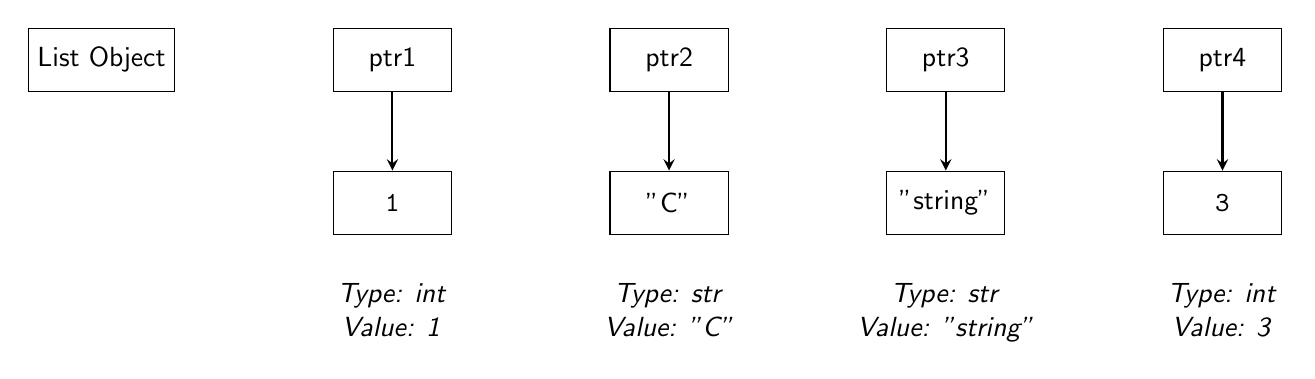
\begin{tikzpicture}[
		node distance=1cm and 2cm,
		every node/.style={font=\sffamily},
		object/.style={rectangle, draw, minimum width=1.5cm, minimum height=0.8cm},
		pointer/.style={-stealth, thick}
		]
		
		% List object array of pointers
		\node[object] (list) {List Object};
		\node[object, right=of list] (ptr1) {ptr1};
		\node[object, right=of ptr1] (ptr2) {ptr2};
		\node[object, right=of ptr2] (ptr3) {ptr3};
		\node[object, right=of ptr3] (ptr4) {ptr4};
		
		% Element nodes
		\node[object, below=of ptr1] (obj1) {\texttt{1}};
		\node[object, below=of ptr2] (obj2) {"C"};
		\node[object, below=of ptr3] (obj3) {"string"};
		\node[object, below=of ptr4] (obj4) {\texttt{3}};
		
		% Metadata (type, ref count)
		\node[below=0.5cm of obj1, align=center] (meta1) {\textit{Type: int}\\ \textit{Value: 1}};
		\node[below=0.5cm of obj2, align=center] (meta2) {\textit{Type: str}\\ \textit{Value: "C"}};
		\node[below=0.5cm of obj3, align=center] (meta3) {\textit{Type: str}\\ \textit{Value: "string"}};
		\node[below=0.5cm of obj4, align=center] (meta4) {\textit{Type: int}\\ \textit{Value: 3}};
		
		% Pointers
		\draw[pointer] (ptr1) -- (obj1.north);
		\draw[pointer] (ptr2) -- (obj2.north);
		\draw[pointer] (ptr3) -- (obj3.north);
		\draw[pointer] (ptr4) -- (obj4.north);
		
	\end{tikzpicture}
	
	\subsection{Static vs. Dynamic Arrays}
	
	Now that you understand how Python lists work behind the scenes, let’s delve into the types of arrays. In the example above, we intentionally constructed a mixed-type Python list. While it mimics array behavior, it lacks the strict type uniformity and memory efficiency of a true array. To understand the distinction, let’s compare \textbf{static} and \textbf{dynamic} arrays.
	
	\subsubsection{Static Arrays}
	
	A \textbf{static array} is one where the size is fixed at compile time. This means that, once declared, the array cannot grow or shrink. The number of elements it can hold must be specified when the array is created.
	For example, in C:
	\begin{lstlisting}[language=C]
		int myArray[10];
	\end{lstlisting}
	This array can hold exactly 10 integers, no more, no less. Static arrays are simple and efficient, but they lack flexibility.
	
	\subsubsection{Dynamic Arrays}
	Dynamic arrays can grow or shrink at runtime. They are super handy when you don’t know the size of the array in advance. Many modern programming languages provide built-in support for dynamic arrays:  
	- Python: `list`  
	- Java: `ArrayList`  
	- C++: `vector`  
	
	Here’s an example in Python:
	\begin{lstlisting}[language=Python]
		my_list = []
		my_list.append(5)  # Add an element
		my_list.append(10) # Add another element
		print(my_list)     # Output: [5, 10]
	\end{lstlisting}
	Despite the ability to resize, dynamic arrays still maintain the basic property of contiguous memory storage, similar to static arrays, which allows for efficient access and manipulation of data.
	\section{Exercises}
	\subsection*{1. Memory Allocation Calculation for Static Arrays}
	\textbf{Description}: Given an array of integers, calculate the total memory required for storing the array. Assume that each integer occupies 4 bytes in memory. Write a program in any language (e.g., C, Python) to compute the memory requirement for an array of size \( N \) where the size of the array is provided by the user.
	
	\textbf{Example}:
	\begin{itemize}
		\item Input: Array size = 15
		\item Output: Total memory required = 60 bytes
	\end{itemize}
	
	\subsection*{2. Memory Representation of Python Lists and JavaScript Arrays}
	\textbf{Description}: Write a detailed comparison of how Python lists and JavaScript arrays are represented in memory. Specifically, explain:
	\begin{itemize}
		\item How elements are stored.
		\item How memory allocation is handled (i.e., contiguously or via pointers).
		\item How elements of different types are stored.
	\end{itemize}
	Provide a visual or pseudo-code representation of the memory layout of a mixed-type list in Python and a similar array in JavaScript.
	
	\subsection*{3. Dynamic Array Resizing in Python}
	\textbf{Description}: Implement a Python class that simulates the behavior of a dynamic array (like Python’s \texttt{list}). The class should support:
	\begin{itemize}
		\item Appending elements.
		\item Automatically resizing when the array exceeds its current capacity.
		\item Printing the current capacity of the array and the number of elements it holds.
	\end{itemize}
	\textbf{Challenge}: Try optimizing the resizing mechanism (e.g., doubling the size, etc.) and analyze the time complexity for different operations.
	
	\subsection*{4. Implementing a Static Array in C with Bounds Checking}
	\textbf{Description}: Implement a static array in C where the size is fixed at compile time. Add bounds checking to prevent out-of-bounds access. The array should allow for basic operations like insertion, deletion, and retrieval. Implement a simple program where the user can interactively choose operations on the array (e.g., insert an element, retrieve an element, etc.).
	
	\textbf{Challenge}: Implement custom error handling for out-of-bounds access and demonstrate how different types of memory issues (e.g., stack overflow, segmentation faults) might arise when bounds checking is not in place.
	
	\subsection*{5. Simulating Mixed-Type Arrays in a Statically Typed Language (e.g., C++)}
	\textbf{Description}: Write a program in C++ that simulates a mixed-type array by using \texttt{void*} pointers (which can point to any type). The program should:
	\begin{itemize}
		\item Create an array where each element can hold a different type (e.g., integer, float, string).
		\item Store the actual values in a struct that includes a pointer to the data and the type information (e.g., an enum representing the data type).
		\item Write functions to add, remove, and display elements, ensuring type safety by checking the stored type at runtime.
	\end{itemize}
	
	\textbf{Challenge}: Implement proper memory management (e.g., freeing memory after use) and demonstrate the trade-offs between type safety and flexibility when working with mixed-type collections in statically typed languages.
	
	\chapter{Basics of Array Operations}
	In the previous chapter, we uncovered how arrays provide constant-time \(O(1)\) access to elements through indexing and how their contiguous memory allocation ensures efficient use of computational resources, such as caches. These qualities make arrays highly suitable for a wide spectrum of tasks, ranging from simple data storage to complex algorithmic processes. However, their usefulness extends far beyond storage; arrays serve as a canvas upon which a diverse set of operations—traversal, insertion, deletion, searching, sorting, and access—can be performed with elegance and precision.\\
	At the same time, arrays are not without limitations. Static arrays, for instance, require predefined sizes, which can lead to over- or under-utilization of memory, while dynamic arrays, although more flexible, may incur overhead during resizing operations. These trade-offs make it imperative to not only understand how arrays function but also to master the operations they support, so you can wield this data structure effectively in different scenarios. This chapter is a journey into the practical aspects of working with arrays. From understanding how to traverse an array with precision to implementing advanced sorting techniques, each section will build upon the previous ones, reinforcing your skills step by step.\\ Let us now begin by exploring the first operation: \textbf{Traversal}, the cornerstone of working with arrays.
	\section{Traversal Operation}
	Traversal is the most fundamental operation you can perform on an array. It involves systematically accessing and processing each element in the array, either to perform computations, display elements, or manipulate their values. Regardless of the programming context, traversal serves as the gateway to more complex operations like searching, sorting, and even data transformation.\\The simplicity of traversal in arrays stems from their contiguous memory layout. This predictable arrangement of elements allows for efficient and orderly processing of data. By iterating sequentially through the array, you can ensure that all elements are systematically accessed and utilized, making traversal both reliable and straightforward.\\Whether the task involves printing elements, calculating their sum, or applying a transformation, array traversal follows a structured approach that guarantees no element is overlooked. This operation unlocks the potential of arrays by enabling full access to their contents for analysis and manipulation.  In essence, traversal provides the mechanism to fully utilize the power of arrays by making their contents accessible and manipulatable. Whether you are iterating through a list of student scores, processing data from a sensor, or applying operations to a sequence of characters in a string, traversal is often the first step in achieving your objective.
	\subsection{Loop Counter in Array Traversal} 
	\subsection{Example in C}
	\subsection{Traversing a 1D Array Within Upper and Lower Bounds}
	\subsection{ Example in Pseudocode}
	\subsection{Traversing a 1D Array Without Explicit Bounds}
	\subsection{Traversal with Initialization}
	\subsection{Algorithm for General Traversal of Linear Array}
	\section{Insertion Operation}
	\subsection*{Algorithm for Insertion}
	\section{Deletion Operation}
	\subsection*{Algorithm for Deletion}
	\section{Search Operation}
	\subsection*{Algorithm for Linear Search}
	\subsection*{Algorithm for Binary Search}
	\section{Sorting Operation}
	\subsection*{Common Sorting Algorithms}
	\section{Access Operation}
	\subsection*{Access Technique}
	\chapter{Types and Representations of Arrays}
	\section{Chomsky}
	\section{Types}
	\section{Abstract Arrays}
	\chapter{Memory Layout and Storage}
	\section{Memory Layout of Arrays}
	\section{Memory Segmentation and Bounds Checking}
	\subsection{Memory Segmentation}
	\subsubsection{Hardware Implementation}
	\subsubsection{Segmentation without Paging}
	\subsubsection{Segmentation with Paging}
	\subsubsection{Historical Implementations}
	\subsubsection{x86 Architecture}
	\subsection{Index-Bounds Checking}
	\subsubsection{Range Checking}
	\subsubsection{Index Checking}
	\subsubsection{Hardware Bounds Checking}
	\subsubsection{Support in High-Level Programming Languages}
	\subsubsection{Buffer Overflow}
	\subsubsection{Integer Overflow}
	\chapter{Development of Array Indexing}
	\subsection{Address Calculation}
	\subsubsection{Address Calculation for Multi-dimensional Arrays}
	\subsubsection{One-Dimensional Array}
	\subsubsection{Two-Dimensional Array}
	\subsubsection{Three-Dimensional Array}
	\subsubsection{Generalizing to a k-Dimensional Array}
	\subsubsection{Examples}
	\chapter{Array Algorithms}
	\section{Sorting Algorithms}
	\section{Searching Algorithms}
	\section{Array Manipulation Algorithms}
	\section{Dynamic Programming and Arrays}
	\chapter{Practical and Advanced Topics}
	\section{Self-Modifying Code in Early Computers}
	\section{Common Array Algorithms}
	\section{Performance Considerations}
	\section{Practical Applications of Arrays}
	\section{Future Trends in Array Handling}
	\chapter{Implementing Arrays in Low-Level Languages}
	\chapter{Static Arrays}
	\section{Single-Dimensional Arrays}
	\subsection{Declaration and Initialization}
	\subsection{Accessing Elements}
	\subsection{Iterating Through an Array}
	\subsection{Common Operations}
	\subsubsection{Insertion}
	\subsubsection{Deletion}
	\subsubsection{Searching}
	\subsection{Memory Considerations}
	\section{Multi-Dimensional Arrays}
	\subsection{2D Arrays}
	\subsubsection{Declaration and Initialization}
	\subsubsection{Accessing Elements}
	\subsubsection{Iterating Through a 2D Array}
	\subsection{3D Arrays and Higher Dimensions}
	\subsubsection{Declaration and Initialization}
	\subsubsection{Accessing Elements}
	\subsubsection{Use Cases and Applications}
	\chapter{Dynamic Arrays}
	\section{Introduction to Dynamic Arrays}
	\subsection{Definition and Overview}
	\subsection{Comparison with Static Arrays}
	
	\section{Single-Dimensional Dynamic Arrays}
	\subsection{Using \texttt{malloc} and \texttt{calloc} in C}
	\subsection{Resizing Arrays with \texttt{realloc}}
	\subsection{Using \texttt{ArrayList} in Java}
	\subsection{Using \texttt{Vector} in C++}
	\subsection{Using \texttt{List} in Python}
	
	\section{Multi-Dimensional Dynamic Arrays}
	\subsection{2D Dynamic Arrays}
	\subsubsection{Creating and Resizing 2D Arrays}
	\subsection{3D and Higher Dimensions}
	\subsubsection{Memory Allocation Techniques}
	\subsubsection{Use Cases and Applications}
	
	\chapter{Advanced Topics in Arrays}
	
	\section{Array Algorithms}
	\subsection{Sorting Algorithms}
	\subsubsection{Bubble Sort}
	\subsubsection{Merge Sort}
	\subsection{Searching Algorithms}
	\subsubsection{Linear Search}
	\subsubsection{Binary Search}
	
	\section{Memory Management in Arrays}
	\subsection{Static vs. Dynamic Memory}
	\subsection{Optimizing Memory Usage}
	
	\section{Handling Large Data Sets}
	\subsection{Efficient Storage Techniques}
	\subsection{Using Arrays in Big Data Applications}
	
	\section{Parallel Processing with Arrays}
	\subsection{Introduction to Parallel Arrays}
	\subsection{Applications in GPU Programming}
	
	\section{Sparse Arrays}
	\subsection{Representation and Usage}
	\subsection{Applications in Data Compression}
	\section{Multidimensional Arrays}
	\section{Jagged Arrays}
	\section{Sparse Arrays}
	\section{Array of Structures vs. Structure of Arrays}
	\section{Array-Based Data Structures}
	
	\chapter{Arrays in Theoretical Computing Paradigms}
	
	\section{Introduction to Theoretical Computing Paradigms}
	\section{Arrays in Turing Machines}
	\section{Arrays in Cellular Automata}
	\section{Arrays in Cellular Automata}
	\section{Arrays in Quantum Computing}
	\section{Arrays in Neural Network Simulations}
	\section{Arrays in Automata Theory}
	\section{Arrays in Hypercomputation Models}
	\section{The Lambda Calculus Perspective on Arrays}
	\section{Arrays in Novel Computational Models}
	
	\chapter{Specialized Arrays and Applications}
	\section{Circular Buffers}
	\section{Circular Arrays}
	\subsection{Implementation and Use Cases}
	\subsection{Applications in Buffer Management}
	
	\section{Dynamic Buffering and Arrays}
	\subsection{Dynamic Circular Buffers}
	\subsection{Handling Streaming Data}
	
	\section{Jagged Arrays}
	\subsection{Definition and Usage}
	\subsection{Applications in Database Management}
	
	\section{Bit Arrays (Bitsets)}
	\subsection{Introduction and Representation}
	\subsection{Applications in Cryptography}
	\section{Circular Buffers}
	\section{Priority Queues}
	\section{Hash Tables}
	\section{Bloom Filters}
	\section{Bit Arrays and Bit Vectors}
	
	\chapter{Linked Lists}
	\section{Overview}
	\section{Singly Linked Lists}
	\section{Doubly Linked Lists}
	\section{Circular Linked Lists}
	\section{Comparison with Arrays}
	
	\chapter{Array-Based Algorithms}
	\section{Sorting Algorithms}
	\section{Searching Algorithms}
	\section{Array Manipulation Algorithms}
	\section{Dynamic Programming and Arrays}
	
	\chapter{Performance Analysis}
	\section{Time Complexity of Array Operations}
	\section{Space Complexity Considerations}
	\section{Cache Performance and Optimization}
	
	\chapter{Memory Management}
	\section{Memory Allocation Strategies}
	\section{Garbage Collection}
	\section{Manual Memory Management in Low-Level Languages}
	
	\chapter{Error Handling and Debugging}
	\section{Common Errors with Arrays}
	\section{Bounds Checking Techniques}
	\section{Debugging Tools and Strategies}
	
	\chapter{Optimization Techniques for Arrays}
	\section{Optimizing Array Traversal}
	\section{Minimizing Cache Misses}
	\section{Loop Unrolling}
	\section{Vectorization}
	\section{Memory Access Patterns}
	\section{Reducing Memory Fragmentation}
	
	\chapter{Concurrency and Parallelism}
	\section{Concurrent Array Access}
	\section{Parallel Array Processing}
	\section{Synchronization Techniques}
	
	\chapter{Applications in Modern Software Development}
	\section{Arrays in Graphics and Game Development}
	\section{Arrays in Scientific Computing}
	\section{Arrays in Data Analysis and Machine Learning}
	\section{Arrays in Embedded Systems}
	
	\chapter{Arrays in High-Performance Computing (HPC)}
	\section{Introduction to HPC Arrays}
	\section{Distributed Arrays}
	\section{Parallel Processing with Arrays}
	\section{Arrays in GPU Computing}
	\section{Multi-threaded Array Operations}
	\section{Handling Arrays in Cloud Computing}
	
	\chapter{Arrays in Functional Programming}
	\section{Immutable Arrays}
	\section{Persistent Arrays}
	\section{Arrays in Functional Languages (Haskell, Erlang, etc.)}
	\section{Functional Array Operations}
	
	\chapter{Arrays in Machine Learning and Data Science}
	\section{Numerical Arrays}
	\section{Handling Large Datasets with Arrays}
	\section{Arrays in Tensor Operations}
	\section{Arrays in Dataframes}
	\section{Optimization of Array-Based Algorithms in ML}
	
	\chapter{Advanced Memory Management in Arrays}
	\section{Memory Pools}
	\section{Dynamic Memory Allocation Strategies}
	
	\chapter{Data Structures Derived from Arrays}
	\section{Stacks}
	\section{Queues}
	\section{Heaps}
	\section{Hash Tables}
	\section{Trees Implemented Using Arrays}
	\section{Graphs Implemented Using Arrays}
	\section{Dynamic Arrays as Building Blocks}
	
	\chapter{Best Practices and Common Pitfalls in Array Usage}
	\section{Avoiding Out-of-Bounds Errors}
	\section{Efficient Initialization}
	\section{Choosing the Right Array Type}
	\section{Debugging and Testing Arrays}
	\section{Avoiding Memory Leaks}
	\section{Ensuring Portability Across Platforms}
	
	\chapter{Historical Perspectives and Evolution}
	\section{Custom Memory Allocators}\section{Early Implementations}
	\section{Array Storage on Disk}\section{Evolution of Array Data Structures}
	\section{Impact on Programming Languages and Paradigms}
	
	\chapter{Future Trends in Array Handling}
	\section{Emerging Data Structures}
	\section{Quantum Computing and Arrays}
	\section{Bioinformatics Applications}
	\section{Big Data and Arrays}
	\section{Arrays in Emerging Programming Paradigms}
	\chapter{Appendices}
	\section{Glossary of Terms}
	\section{Bibliography}
	\section{Index}
	
% References
\printbibliography[heading=bibintoc]

% Index
\printindex
\end{document}